\documentclass[12pt]{article}


\usepackage[margin=1in]{geometry}
\usepackage{amsmath}
\usepackage{amsfonts}
\usepackage{graphicx}      % include this line if your document contains figures
\usepackage{enumerate}
\usepackage{cite}
\usepackage{circuitikz}
\usetikzlibrary{patterns}
\usetikzlibrary{shapes.geometric}


\definecolor{msblue}{rgb}{0.357, 0.608, 0.835}
\definecolor{msgreen}{rgb}{0.439, 0.678, 0.278}
\definecolor{msred}{rgb}{0.753, 0, 0}
\definecolor{msyellow}{rgb}{0.984, 0.737, 0.0196}



\title{Figures for Unit 1 - Models and Representations}
\date{\today}
\author{Arne Dankers}


\begin{document}
\maketitle

%\begin{figure}[htb]
%\begin{circuitikz}[american]
%    \draw (0,0) to[isource] (0,3) -- (2,3) to[R] (2,0) -- (0,0);
%\end{circuitikz}
%\end{figure}


\begin{figure}[htb]    
\begin{circuitikz}[american]
    \node[op amp, noinv input up, anchor=+] (OA) at (4,0) {\texttt{OA1}} ;
    \node[label=above:{$v_i$},inner sep=0] (vi) at (0,0) {};
    \node[inner sep=0] (r2) at (6.5,1.5) {};
    \draw (vi) to[short, o-] (1,0);
    \draw (1,0) to[R=$R_1$] (OA.+);
    \draw (3.5,0) -- (3.5,1.5) to[R=$R_2$] (r2) -- (r2 |- OA.out);
    \draw (OA.out) to[short,-o] ++(1,0) node[above]{$v_o$};
    \draw (OA.-) -- ++(0,-1) node[ground]{};
\end{circuitikz}
\end{figure}


\begin{figure}[htb]    
    \begin{circuitikz}[american]
        \node[op amp, noinv input up, anchor=+] (OA) at (5,0) {\texttt{OA1}} ;
        \node[label=above:{$v_i$},inner sep=0] (vi) at (0,0) {};
        \node[inner sep=0] (r2) at (7.5,1.5) {};
        \draw (vi) to[short, o-] (1,0);
        \draw (1,0) -- (1,-0.75) to[R=$R_1$] (3,-0.75) -- (3,0) -- (OA.+);
        \draw (1,0) -- (1,0.75) to[C=$C_1$] (3,0.75) -- (3,0);
        \draw (3.5,0) -- (3.5,1.5) to[R=$R_2$] (5.5,1.5) to[C=$C_2$] (r2) -- (r2 |- OA.out);
        
        \draw (OA.out) to[short,-o] ++(1,0) node[above]{$v_o$};
        \draw (OA.-) -- ++(0,-1) node[ground]{};
    \end{circuitikz}
\end{figure}
    

\begin{figure}[htb]
    \begin{circuitikz}
        \pattern[pattern=north east lines] (0,0) rectangle (7,.25);
        \draw[thick] (0,0.25) -- (7,0.25);
        \draw (3,0.25) to[spring,l=$k$] (3,2);
        \draw (4,0.25) to[damper,l_=$b$] (4,2);
        \draw[fill=gray!40] (2.5,2) rectangle (4.5,3);
        \node at (3.5,2.5) {$m$};
        \draw[thick, ->] (3.5,4) -- (3.5,3);
        \node at (3.75,3.75) {$F$};
    \end{circuitikz}
\end{figure}


\begin{figure}[htb]
    \begin{circuitikz}
        \pattern[pattern=north east lines] (0,0) rectangle (16,0.25);
        \draw[thick] (0,0.25) -- (16,0.25);

        \draw[fill=gray!40] (0.25,0.5) rectangle (3.75,1.5);
        \draw[fill=gray!40] (4.25,0.5) rectangle (7.75,1.5);
        \draw[fill=gray!40] (8.25,0.5) rectangle (11.75,1.5);
        \draw[fill=gray!40] (12.25,0.5) -- (15.75,0.5) -- (15.75,1.25) -- (15.5,1.25) -- (15.25,1.5) -- (12.25,1.5) -- cycle;
        \draw (0.375,0.375) circle (0.125);
        \draw (0.625,0.375) circle (0.125);
        \draw (3.375,0.375) circle (0.125);
        \draw (3.625,0.375) circle (0.125);
        \draw (4.375,0.375) circle (0.125);
        \draw (4.625,0.375) circle (0.125);
        \draw (7.375,0.375) circle (0.125);
        \draw (7.625,0.375) circle (0.125);
        \draw (8.375,0.375) circle (0.125);
        \draw (8.625,0.375) circle (0.125);
        \draw (11.375,0.375) circle (0.125);
        \draw (11.625,0.375) circle (0.125);
        \draw (12.375,0.375) circle (0.125);
        \draw (12.625,0.375) circle (0.125);
        \draw (15.375,0.375) circle (0.125);
        \draw (15.625,0.375) circle (0.125);
        \draw[fill=white] (15.25,1.5) -- (15.25,1.25) -- (15.5,1.25) -- cycle;
        \draw[fill=gray!40] (12.15,1.5) rectangle (13.5,1.6);
        \draw[fill=gray!40] (14,1.5) rectangle (15.3,1.6);        
        \draw[fill=white] (14.5,1.25) rectangle (15.15,1.45);
        \draw (12.25,1) -- (15.75,1);

        \draw (3.75,0.6) -- (4.25,0.6);
        \draw (7.75,0.6) -- (8.25,0.6);
        \draw (11.75,0.6) -- (12.25,0.6);
    \end{circuitikz}
\end{figure}



\begin{figure}[htb]
    \begin{circuitikz}
        \pattern[pattern=north east lines] (0,-0.25) rectangle (16,0);
        \draw[thick] (0,0) -- (16,0);

        \draw[fill=gray!40] (1,0.5) rectangle (3,2.5);
        \draw[fill=gray!40] (5,0.5) rectangle (7,2.5);
        \draw[fill=gray!40] (9,0.5) rectangle (11,2.5);
        \draw[fill=gray!40] (13,0.5) rectangle (15,2.5);
        \draw (1.5,0.25) circle (0.25);
        \draw (2.5,0.25) circle (0.25);
        \draw (5.5,0.25) circle (0.25);
        \draw (6.5,0.25) circle (0.25);
        \draw (9.5,0.25) circle (0.25);
        \draw (10.5,0.25) circle (0.25);
        \draw (13.5,0.25) circle (0.25);
        \draw (14.5,0.25) circle (0.25);


        \node at (2,1.5) {$m_4$};
        \node at (6,1.5) {$m_3$};
        \node at (10,1.5) {$m_2$};
        \node at (14,1.5) {$m_1$};

        \draw (3,2) to[spring,l=$k_3$] (5,2);
        \draw (3,1) to[damper,l_=$b_3$] (5,1);
 
        \draw (7,2) to[spring,l=$k_2$] (9,2);
        \draw (7,1) to[damper,l_=$b_2$] (9,1);
 
        \draw (11,2) to[spring,l=$k_1$] (13,2);
        \draw (11,1) to[damper,l_=$b_1$] (13,1);
 
        
        \draw[thick, ->] (15,1.5) -- (16,1.5);
        \node at (16.5,1.5) {$F_1$};
    \end{circuitikz}
\end{figure}



\begin{figure}[htb]
    \begin{circuitikz}

        \draw (1,0.5) rectangle (3,2.5);
        \draw (5,0.5) rectangle (7,2.5);
        \draw (9,0.5) rectangle (11,2.5);
        \draw (13,0.5) rectangle (15,2.5);
        \node at (2,1.5) {$m_4$};
        \node at (6,1.5) {$m_3$};
        \node at (10,1.5) {$m_2$};
        \node at (14,1.5) {$m_1$};

        \node at (0,1) {$F_{f_4}$};

        \draw[thick,->] (3,1.5) -- (3.5,1.5);
        \draw[thick,->] (3,2) -- (3.5,2);
        \draw[thick,->] (1,1) -- (0.5,1);
        
        \node at (4,1) {$F_{f_3}$};
        \node at (4,1.5) {$F_{d_3}$};
        \node at (4,2) {$F_{s_3}$};
 
        \draw[thick,->] (5,2) -- (4.5,2);
        \draw[thick,->] (5,1) -- (4.5,1);
        \draw[thick,->] (5,1.5) -- (4.5,1.5);
        \draw[thick,->] (7,1.5) -- (7.5,1.5);
        \draw[thick,->] (7,2) -- (7.5,2);

        \node at (8,1) {$F_{f_2}$};
        \node at (8,1.5) {$F_{d_2}$};
        \node at (8,2) {$F_{s_2}$};
 
        \draw[thick,->] (9,2) -- (8.5,2);
        \draw[thick,->] (9,1) -- (8.5,1);
        \draw[thick,->] (9,1.5) -- (8.5,1.5);
        \draw[thick,->] (11,1.5) -- (11.5,1.5);
        \draw[thick,->] (11,2) -- (11.5,2);

        \node at (12,1) {$F_{f_1}$};
        \node at (12,1.5) {$F_{d_1}$};
        \node at (12,2) {$F_{s_1}$};
 
        \draw[thick,->] (13,2) -- (12.5,2);
        \draw[thick,->] (13,1) -- (12.5,1);
        \draw[thick,->] (13,1.5) -- (12.5,1.5);
        \draw[thick,->] (15,1.5) -- (15.5,1.5);
        \node at (16,1.5) {$F_1$};

        \draw[thick,->] (2,0) -- (2,0.5);
        \draw[thick,->] (6,0) -- (6,0.5);
        \draw[thick,->] (10,0) -- (10,0.5);
        \draw[thick,->] (14,0) -- (14,0.5);

        \node at (2,-0.5) {$F_{N_1}$};
        \node at (6,-0.5) {$F_{N_2}$};
        \node at (10,-0.5) {$F_{N_3}$};
        \node at (14,-0.5) {$F_{N_4}$};


    \end{circuitikz}
\end{figure}


\begin{figure}[htb]
    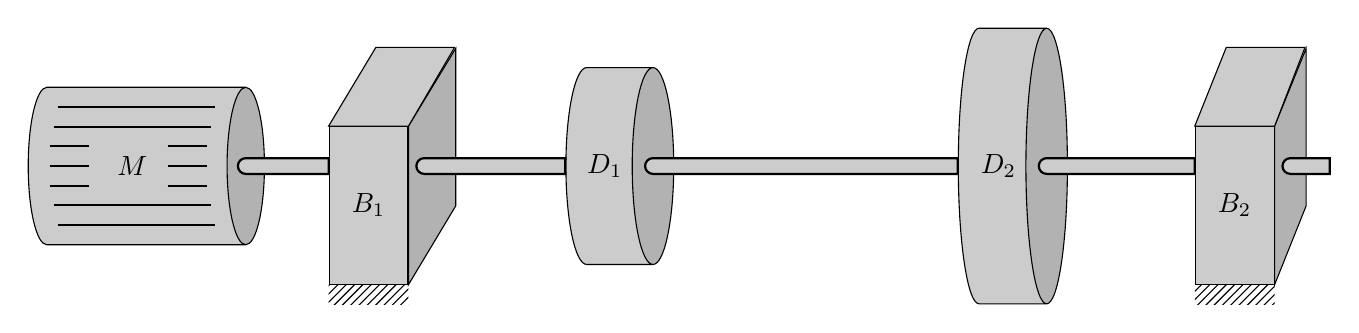
\begin{tikzpicture}
 
        \node[cylinder, 
            draw = black,
            cylinder uses custom fill, 
            cylinder body fill = gray!40, 
            cylinder end fill = gray!60,
            minimum width = 2.5cm,
            minimum height = 1cm] (d1) at (0,0) {$D_1$};

        \node[cylinder, 
            draw = black,
            cylinder uses custom fill, 
            cylinder body fill = gray!40, 
            cylinder end fill = gray!60,
            minimum width = 3.5cm,
            minimum height = 1cm] (d2) at (5,0) {$D_2$};

        \node[rectangle, minimum width=1cm,minimum height=2cm,draw,fill=gray!40] (b2) at (8,-0.5) {$B_2$};
        \draw[fill=gray!60] (b2.south east) -- ++(0.4,1) -- ++(0,2) -- (b2.north east) -- cycle;
        \draw[fill=gray!40] (b2.north west) -- ++(0.4,1) -- ++(1,0) -- (b2.north east) -- cycle;
        \pattern[pattern=north east lines] ($(b2.south west)+(0,-0.25)$) rectangle (b2.south east);

        \node[rectangle, minimum width=1cm,minimum height=2cm,draw,fill=gray!40] (b1) at (-3,-0.5) {$B_1$};
        \draw[fill=gray!60] (b1.south east) -- ++(0.6,1) -- ++(0,2) -- (b1.north east) -- cycle;
        \draw[fill=gray!40] (b1.north west) -- ++(0.6,1) -- ++(1,0) -- (b1.north east) -- cycle;
        \pattern[pattern=north east lines] ($(b1.south west)+(0,-0.25)$) rectangle (b1.south east);

        \node[cylinder, 
            draw = black,
            cylinder uses custom fill, 
            cylinder body fill = gray!40, 
            cylinder end fill = gray!60,
            minimum width = 2cm,
            minimum height = 3cm] (m) at (-6,0) {$M$};
        \draw[thick] (-6.95,0.75) -- (-4.95,0.75); 
        \draw[thick] (-7,0.5) -- (-5,0.5); 
        \draw[thick] (-7.05,0.25) -- (-6.55,0.25); 
        \draw[thick] (-7.05,0) -- (-6.55,0); 
        \draw[thick] (-7.05,-0.25) -- (-6.55,-0.25); 
        \draw[thick] (-5.55,0.25) -- (-5.05,0.25); 
        \draw[thick] (-5.55,0) -- (-5.05,0); 
        \draw[thick] (-5.55,-0.25) -- (-5.05,-0.25); 

        \draw[thick] (-7,-0.5) -- (-5,-0.5); 
        \draw[thick] (-6.95,-0.75) -- (-4.95,-0.75); 
        

        %\draw[thick] ($(d1.before top |- d1.east) + (0,0.1)$) -- ($(d2.west)+(0,0.1)$);
        %\draw[thick] ($(d1.before top |- d1.east) - (0,0.1)$) -- ($(d2.west)-(0,0.1)$);
        \draw[thick,fill=gray!40] ($(d1.before top |- d1.east) - (0,0.1)$) arc (270:90:0.1) -- ($(d2.west)+(0,0.1)$) -- ($(d2.west)-(0,0.1)$) -- cycle;

        \draw[thick,fill=gray!40] ($(d2.before top |- d2.east) - (0,0.1)$) arc (270:90:0.1) -- ($(b2.west)+(0,0.1+0.5)$) -- ($(b2.west)+(0,-0.1+0.5)$) -- cycle;

        \draw[thick,fill=gray!40] ($(b2.east) + (0.2,0.5-0.1)$) arc (270:90:0.1) -- ++(0.5,0) -- ++(0,-0.2) -- cycle;

        \draw[thick,fill=gray!40] ($(b1.east) + (0.2,0.5-0.1)$) arc (270:90:0.1) -- ($(d1.west)+(0,0.1)$) -- ++(0,-0.2) -- cycle;

        \draw[thick,fill=gray!40] ($(m.before top |- m.east) - (0,0.1)$) arc (270:90:0.1) -- ($(b1.west)+(0,0.1+0.5)$) -- ($(b1.west)+(0,-0.1+0.5)$) -- cycle;



    \end{tikzpicture}
\end{figure}


\begin{figure}[htp]
    \begin{circuitikz}
        \node (T) at (0,0) {};
        \node[draw,rectangle,minimum size=2cm] (J1) at (4,0) {$J_1$};
        \node[draw,rectangle,minimum size=2cm] (J2) at (8,0) {$J_2$};
        \node at (-0.5,0.5) {$T_M$};

        \draw (T) to[damper,l=$b_1$] (J1);
        \draw (J1) to[spring,l=$k$] (J2);
        \draw (J2) to[damper,l=$b_2$] (12,0); 
        \draw[->] ($(T) + (0,-0.125)$) arc (330:30:0.25);  
    \end{circuitikz}
\end{figure}



\begin{figure}[htp]
    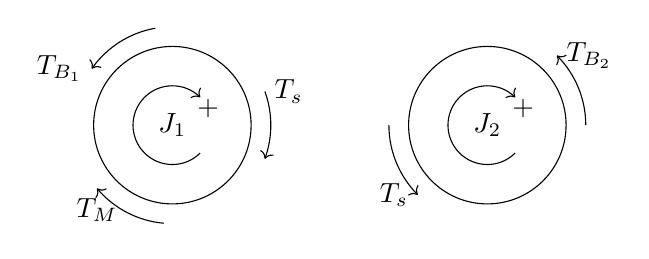
\begin{tikzpicture}
        \node[circle,draw,minimum size=2cm] (J1) at (0,0) {$J_1$};
        \node[circle,draw,minimum size=2cm] (J2) at (4,0) {$J_2$};

        \draw[<-] (340:1.25) arc (340:380:1.25) node[right]{$T_{s}$};
        \draw[->] (100:1.25) arc (100:145:1.25) node[left]{$T_{B_1}$};
        \draw[->] (265:1.25) arc (265:220:1.25) node[below]{$T_M$};
        \draw[->] (315:0.5) arc (315:45:0.5);
        \node at (25:0.5) {$+$};
        \draw[->] (5.25cm,0) arc (0:45:1.25) node[right]{$T_{B_2}$};
        \draw[->] (2.75,0) arc (180:225:1.25) node[left]{$T_{s}$};
        \draw[->] ($(4,0)+(315:0.5)$) arc (315:45:0.5);
        \node at ($(4,0)+(25:0.5)$) {$+$};

    \end{tikzpicture}
\end{figure}



\begin{figure}[htb]
    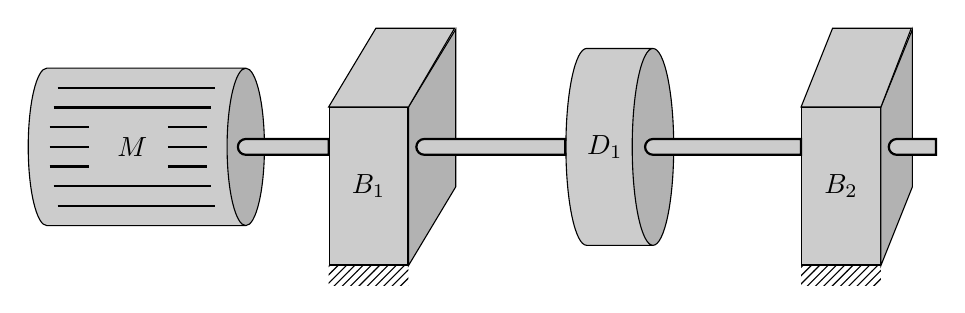
\begin{tikzpicture}
 
        \node[cylinder, 
            draw = black,
            cylinder uses custom fill, 
            cylinder body fill = gray!40, 
            cylinder end fill = gray!60,
            minimum width = 2.5cm,
            minimum height = 1cm] (d1) at (0,0) {$D_1$};

        \node[rectangle, minimum width=1cm,minimum height=2cm,draw,fill=gray!40] (b2) at (3,-0.5) {$B_2$};
        \draw[fill=gray!60] (b2.south east) -- ++(0.4,1) -- ++(0,2) -- (b2.north east) -- cycle;
        \draw[fill=gray!40] (b2.north west) -- ++(0.4,1) -- ++(1,0) -- (b2.north east) -- cycle;
        \pattern[pattern=north east lines] ($(b2.south west)+(0,-0.25)$) rectangle (b2.south east);

        \node[rectangle, minimum width=1cm,minimum height=2cm,draw,fill=gray!40] (b1) at (-3,-0.5) {$B_1$};
        \draw[fill=gray!60] (b1.south east) -- ++(0.6,1) -- ++(0,2) -- (b1.north east) -- cycle;
        \draw[fill=gray!40] (b1.north west) -- ++(0.6,1) -- ++(1,0) -- (b1.north east) -- cycle;
        \pattern[pattern=north east lines] ($(b1.south west)+(0,-0.25)$) rectangle (b1.south east);

        \node[cylinder, 
            draw = black,
            cylinder uses custom fill, 
            cylinder body fill = gray!40, 
            cylinder end fill = gray!60,
            minimum width = 2cm,
            minimum height = 3cm] (m) at (-6,0) {$M$};
        \draw[thick] (-6.95,0.75) -- (-4.95,0.75); 
        \draw[thick] (-7,0.5) -- (-5,0.5); 
        \draw[thick] (-7.05,0.25) -- (-6.55,0.25); 
        \draw[thick] (-7.05,0) -- (-6.55,0); 
        \draw[thick] (-7.05,-0.25) -- (-6.55,-0.25); 
        \draw[thick] (-5.55,0.25) -- (-5.05,0.25); 
        \draw[thick] (-5.55,0) -- (-5.05,0); 
        \draw[thick] (-5.55,-0.25) -- (-5.05,-0.25); 

        \draw[thick] (-7,-0.5) -- (-5,-0.5); 
        \draw[thick] (-6.95,-0.75) -- (-4.95,-0.75); 
        

        %\draw[thick] ($(d1.before top |- d1.east) + (0,0.1)$) -- ($(d2.west)+(0,0.1)$);
        %\draw[thick] ($(d1.before top |- d1.east) - (0,0.1)$) -- ($(d2.west)-(0,0.1)$);
        \draw[thick,fill=gray!40] ($(d1.before top |- d1.east) - (0,0.1)$) arc (270:90:0.1) -- ($(b2.west)+(0,0.1+0.5)$) -- ($(b2.west)+(0,-0.1+0.5)$) -- cycle;

        \draw[thick,fill=gray!40] ($(b2.east) + (0.2,0.5-0.1)$) arc (270:90:0.1) -- ++(0.5,0) -- ++(0,-0.2) -- cycle;

        \draw[thick,fill=gray!40] ($(b1.east) + (0.2,0.5-0.1)$) arc (270:90:0.1) -- ($(d1.west)+(0,0.1)$) -- ++(0,-0.2) -- cycle;

        \draw[thick,fill=gray!40] ($(m.before top |- m.east) - (0,0.1)$) arc (270:90:0.1) -- ($(b1.west)+(0,0.1+0.5)$) -- ($(b1.west)+(0,-0.1+0.5)$) -- cycle;
    \end{tikzpicture}
\end{figure}


\begin{figure}[htp]
    \begin{circuitikz}
        \node (T) at (0,0) {};
        \node[draw,rectangle,minimum size=2cm] (J1) at (6,0) {$J_1$};        
        \draw (T) to[damper,l=$b_1$] (2,0) to[spring,l=$k_1$] (J1);
        \draw (J1) to[spring,l=$k_2$] (10,0) to[damper,l=$b_2$] (12,0); 


        \node at (-0.5,0.5) {$\theta_1$};
        \node at (12.75,0.5) {$\theta_2$};
        \draw[->] ($(T) + (0,-0.125)$) arc (330:30:0.25);  
        \draw[->] ($(12.75,0) + (0,-0.125)$) arc (330:30:0.25);  

    \end{circuitikz}
\end{figure}



\begin{figure}[htp]
    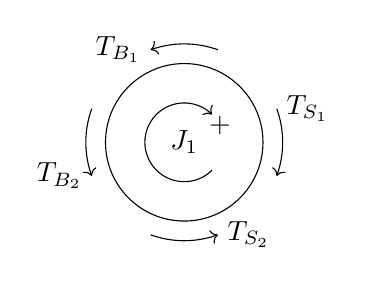
\begin{tikzpicture}
        \node[circle,draw,minimum size=2cm] (J1) at (0,0) {$J_1$};
        \draw[<-] (340:1.25) arc (340:380:1.25) node[right]{$T_{S_1}$};
        \draw[->] (70:1.25) arc (70:110:1.25) node[left]{$T_{B_1}$};
        \draw[->] (160:1.25) arc (160:200:1.25) node[left]{$T_{B_2}$};
        \draw[->] (250:1.25) arc (250:290:1.25) node[right]{$T_{S_2}$};
        \draw[->] (315:0.5) arc (315:45:0.5);
        \node at (25:0.5) {$+$};
    \end{tikzpicture}
\end{figure}


\begin{figure}[htb]
    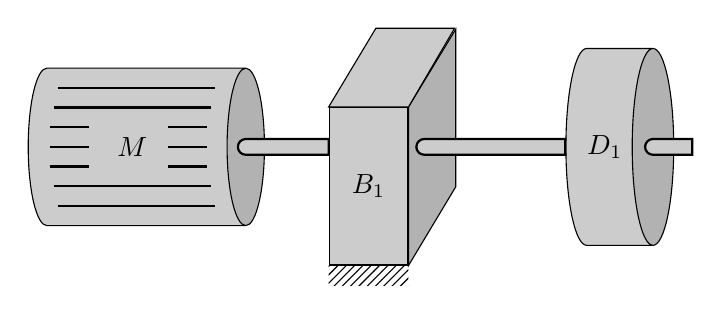
\begin{tikzpicture}
 
        \node[cylinder, 
            draw = black,
            cylinder uses custom fill, 
            cylinder body fill = gray!40, 
            cylinder end fill = gray!60,
            minimum width = 2.5cm,
            minimum height = 1cm] (d1) at (0,0) {$D_1$};

        \node[rectangle, minimum width=1cm,minimum height=2cm,draw,fill=gray!40] (b1) at (-3,-0.5) {$B_1$};
        \draw[fill=gray!60] (b1.south east) -- ++(0.6,1) -- ++(0,2) -- (b1.north east) -- cycle;
        \draw[fill=gray!40] (b1.north west) -- ++(0.6,1) -- ++(1,0) -- (b1.north east) -- cycle;
        \pattern[pattern=north east lines] ($(b1.south west)+(0,-0.25)$) rectangle (b1.south east);

        \node[cylinder, 
            draw = black,
            cylinder uses custom fill, 
            cylinder body fill = gray!40, 
            cylinder end fill = gray!60,
            minimum width = 2cm,
            minimum height = 3cm] (m) at (-6,0) {$M$};
        \draw[thick] (-6.95,0.75) -- (-4.95,0.75); 
        \draw[thick] (-7,0.5) -- (-5,0.5); 
        \draw[thick] (-7.05,0.25) -- (-6.55,0.25); 
        \draw[thick] (-7.05,0) -- (-6.55,0); 
        \draw[thick] (-7.05,-0.25) -- (-6.55,-0.25); 
        \draw[thick] (-5.55,0.25) -- (-5.05,0.25); 
        \draw[thick] (-5.55,0) -- (-5.05,0); 
        \draw[thick] (-5.55,-0.25) -- (-5.05,-0.25); 

        \draw[thick] (-7,-0.5) -- (-5,-0.5); 
        \draw[thick] (-6.95,-0.75) -- (-4.95,-0.75); 
        

        %\draw[thick] ($(d1.before top |- d1.east) + (0,0.1)$) -- ($(d2.west)+(0,0.1)$);
        %\draw[thick] ($(d1.before top |- d1.east) - (0,0.1)$) -- ($(d2.west)-(0,0.1)$);
        \draw[thick,fill=gray!40] ($(d1.before top |- d1.east) - (0,0.1)$) arc (270:90:0.1) -- ++(0.5,0) -- ++(0,-0.2) -- cycle;

        \draw[thick,fill=gray!40] ($(b1.east) + (0.2,0.5-0.1)$) arc (270:90:0.1) -- ($(d1.west)+(0,0.1)$) -- ++(0,-0.2) -- cycle;

        \draw[thick,fill=gray!40] ($(m.before top |- m.east) - (0,0.1)$) arc (270:90:0.1) -- ($(b1.west)+(0,0.1+0.5)$) -- ($(b1.west)+(0,-0.1+0.5)$) -- cycle;
    \end{tikzpicture}
\end{figure}


\begin{figure}[htp]
    \begin{circuitikz}
        \node (T) at (0,0) {};
        \node[draw,rectangle,minimum size=2cm] (J1) at (6,0) {$J$};        
        \draw (T) to[damper,l=$b$] (2,0) to[spring,l=$k$] (J1); 


        \node at (-0.5,0.5) {$\theta_1$};
        \node at (7.75,0.5) {$\theta_2$};
        \draw[->] ($(T) + (0,-0.125)$) arc (330:30:0.25);  
        \draw[->] ($(7.75,0) + (0,-0.125)$) arc (330:30:0.25);  

    \end{circuitikz}
\end{figure}



\begin{figure}[htp]
    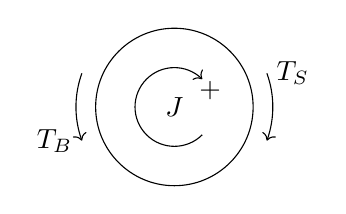
\begin{tikzpicture}
        \node[circle,draw,minimum size=2cm] (J1) at (0,0) {$J$};
        \draw[<-] (340:1.25) arc (340:380:1.25) node[right]{$T_{S}$};
        \draw[->] (160:1.25) arc (160:200:1.25) node[left]{$T_{B}$};
        \draw[->] (315:0.5) arc (315:45:0.5);
        \node at (25:0.5) {$+$};
    \end{tikzpicture}
\end{figure}


\end{document}